% !TeX spellcheck = de_DE
% !TeX document-id = {8f28539b-0e77-467c-988f-5fbde5f3c76b}
% !TeX TXS-program:compile = txs:///pdflatex/[--shell-escape]
\documentclass[accentcolor=tud8b,colorbacktitle,inverttitle,landscape,german,presentation,t]{tudbeamer}
\usepackage[utf8]{inputenc}
\usepackage[ngerman]{babel}
\usepackage{graphicx}
\usepackage{svg}
\usepackage{listings}
\usepackage{tabto}
\usepackage{tikz}
\usepackage{pgfpages}
\usetikzlibrary{shapes}


% notes
%\setbeamertemplate{note page}[plain]
%\setbeameroption{show notes on second screen=right}

% only display outmost section
\setcounter{tocdepth}{2}


\definecolor{darkblue}{rgb}{0,0,.5}
%\hypersetup{colorlinks=true, breaklinks=true, linkcolor=darkblue, menucolor=darkblue, urlcolor=darkblue}
\graphicspath{{media/}}

\lstset{language=sh,basicstyle=\ttfamily\small, keywordstyle=\color{blue!80!black}, identifierstyle=, commentstyle=\color{green!50!black}, stringstyle=\ttfamily,
	tabsize=4, breaklines=true, numbers=left, numberstyle=\small, frame=single, backgroundcolor=\color{blue!3}}

\newcommand{\diffp}[1]{\textcolor{darkgreen}{+} & \textcolor{darkgreen}{#1}}
\newcommand{\diffm}[1]{\textcolor{red}{-} & \textcolor{red}{#1}}
\newcommand{\diffn}[1]{\textcolor{darkgreen}{#1}}
\newcommand{\flownumber}[1]{\textcolor{orange}{#1.}\enspace}

%{\setlength{\tabcolsep}{.2em}

\begin{document}
\title[Git-Workshop]{Wie Git denn das?\\Einführung in die Versionskontrolle mit Git}
\subtitle{Fachschaft Informatik TU Darmstadt}

\author[]{}
\institute[Fachschaft Informatik TU Darmstadt]{Fachschaft Informatik TU Darmstadt}

\logo[1]{
\includegraphics{bildmarke_ohne_rand}}

\date{\today}



\begin{titleframe}
	\makebox(1,28)[]{}
	\begin{figure}[ht]
	\centering
  	
\includegraphics[height=60px]{git_logo}
	\end{figure}

	\vskip0pt plus 1filll
	%\small Vortrag: Steffen Klee
	\vskip -1em
\end{titleframe}

\begin{frame}
\frametitle{Übersicht}
\tableofcontents
\end{frame}


\section{Warum Git?}
		\begin{frame}
			\frametitle{Warum Quellcodeverwaltung?}
				\begin{tikzpicture}[remember picture, note/.style={ellipse callout, fill=red!50}]
    				\node [note=blue!50, text width=3.5cm, opacity=0.90, overlay, callout absolute pointer={(-0.3,-2)}] at (3,-0.2) {Ich habe euch meinen Code doch per E-Mail geschickt.};
  				\end{tikzpicture}
  				\begin{tikzpicture}[remember picture, note/.style={ellipse callout, fill=green!50}]
    				\node [note=blue!50, text width=4cm, opacity=0.90, overlay, callout absolute pointer={(12.3,-2)}] at (8.5,-1.5) {Nein, die andere E-Mail!};
  				\end{tikzpicture}
		\end{frame}

		\begin{frame}
			\frametitle{Warum Quellcodeverwaltung?}
				\begin{tikzpicture}[remember picture, note/.style={ellipse callout, fill=red!50}]
    				\node [note=blue!50, text width=3.5cm, opacity=0.90, overlay, callout absolute pointer={(-0.3,-2)}] at (3,-0.2) {Ich habe euch meinen Code doch per E-Mail geschickt.};
  				\end{tikzpicture}
  				\begin{tikzpicture}[remember picture, note/.style={ellipse callout, fill=green!50}]
    				\node [note=blue!50, text width=4cm, opacity=0.90, overlay, callout absolute pointer={(12.3,-2)}] at (8.5,-1.5) {Nein, die andere E-Mail!};
  				\end{tikzpicture}
  				
  				\begin{tikzpicture}[remember picture, note/.style={ellipse callout, fill=red!50}]
    				\node [note=blue!50, text width=3.5cm, opacity=0.90, overlay, callout absolute pointer={(-0.3,-2)}] at (3,-3) {Jaja, ich lege es gleich in die Cloud.};
  				\end{tikzpicture}
  				\begin{tikzpicture}[remember picture, note/.style={ellipse callout, fill=green!50}]
    				\node [note=blue!50, text width=3.5cm, opacity=0.90, overlay, callout absolute pointer={(12.3,-2)}] at (8.5,-4) {Ach, ihr habt die Datei auch geändert???};
  				\end{tikzpicture}
		\end{frame}
		
		\begin{frame}
			    \frametitle{Warum Quellcodeverwaltung?}
			    	\begin{tikzpicture}[remember picture, note/.style={ellipse callout, fill=yellow!50}]
    				\node [note=blue!50, text width=4.3cm, opacity=0.90, overlay, callout absolute pointer={(3,-4)}] at (6,-2) {Das ging doch mal!\\Wer hat das denn geändert?\\Am liebsten hätte ich wieder den Stand von gestern.};
  				\end{tikzpicture}
		\end{frame}
		
		\begin{frame}
			\frametitle{Darum Quellcodeverwaltung!}
				\begin{itemize}
					\item zentrales Quellcodeverzeichnis
					\item offline (und online)
					\item gleichzeitige Bearbeitung: Lösung von Versionskonflikten
					\item Versionshistorie (Autor, Zeit)
				\end{itemize}
			\vskip 4em
			\begin{block}{Insgesamt:}
				Vereinfachte Zusammenarbeit
			\end{block}
						
		\note{
			- offline verwalten: Dateien vollständig vorhanden\\
			- Versionshistorie:
			\begin{itemize}
				\item Wer hat wann was gemacht?
				\item Wiederherstellung alter Versionen und Rückgängigmachen einzelner Änderungen
			\end{itemize}
		}
		\end{frame}
		\begin{frame}
			\frametitle{Warum Git?}
				\begin{itemize}
					\item weit verbreitet
				% Linux, Eclipse
					\item die im \textit{Open Source}-Bereich oft genutzten Plattformen \textbf{GitLab} und \textbf{GitHub} basieren auf Git
					\item auf \href{https://git.rwth-aachen.de}{https://git.rwth-aachen.de} verfügbar
					\item auf eigenen Servern leicht zu hosten
%					\item[\checkmark] Just do Git!
					\item Alternativen sind zum Beispiel \textbf{Mercurial} und \textbf{SVN}
				\end{itemize}
			
			\note{
				weit verbreitet: Linux, Eclipse
			}
		\end{frame}
		
\section{Funktionsweise}
	 \subsection{Normalfall}
		\begin{frame}
			\frametitle{Funktionsweise}
				\vskip -1em
				\begin{tikzpicture}
					\definecolor{lightblue}{HTML}{7F7FFF}
					\definecolor{darkgreen}{HTML}{00A700}
					% timeline
					\draw[very thick] (0,0) -- (0, 5.9);
					
					% commit diamonds
					\draw<4->[very thick,blue,fill=lightblue] (0,0.6) -- (0.2,0.8) -- (0,1) -- (-0.2,0.8) -- (0,0.6);
					\draw<3->[very thick,blue,fill=lightblue] (0,2.03) -- (0.2,2.23) -- (0,2.43) -- (-0.2,2.23) -- (0,2.03);
					\draw<2->[very thick,blue,fill=lightblue] (0,3.57) -- (0.2,3.77) -- (0,3.97) -- (-0.2,3.77) -- (0,3.57);
					\draw<1->[very thick,blue,fill=lightblue] (0,5) -- (0.2,5.2) -- (0,5.4) -- (-0.2,5.2) -- (0,5);
					
					% commit hashes
					\node<4->[anchor=west] at (-2,0.79) {\texttt{54cdb2c}};
					\node<3->[anchor=west] at (-2,2.22) {\texttt{f39a8c8}};
					\node<2->[anchor=west] at (-2,3.76) {\texttt{7854994}};
					\node<1->[anchor=west] at (-2,5.19) {\texttt{1f42b40}};
					
					% commit message
					\node<4->[anchor=west] at (0.5,0.79) {\textbf{Revert: Implemented add}};
					\node<4->[anchor=west] at (0.5,0.39) {We do not need to implement};
					\node<4->[anchor=west] at (0.5,0.10) { this for the first assignment.};
					\node<3->[anchor=west] at (0.5,2.22) {\textbf{Implemented sub}};
					\node<2->[anchor=west] at (0.5,3.76) {\textbf{Implemented add}};
					\node<2->[anchor=west] at (0.5,3.36) {Solved task 1};
					\node<1->[anchor=west] at (0.5,5.19) {\textbf{Initial commit}};
					
					% commit diffs
					
					%% 1st commit
					\node<1->[draw,fill=white,anchor=west] at (3.5,5.15) {\footnotesize\texttt{
						\begin{tabular}{rl}
							\diffp{int add(int a, int b)\{}\\
							\diffp{// TODO implement}\\
							\diffp{\}}\\
							\diffp{int sub(int a, int b)\{}\\
							\diffp{// TODO implement}\\
							\diffp{\}}
						\end{tabular}}};
						
					%% 2nd commit
					\node<2->[draw,fill=white,anchor=west] at (5,4) {\small\texttt{
						\begin{tabular}{rl}
							&int add(int a, int b)\{\\
							\diffm{// TODO implement} \\
							\diffp{\hspace*{0.5cm}return a + b;}\\
							&\}
						\end{tabular}}};
	
					%% 3rd commit
					\node<3->[draw,fill=white,anchor=west] at (3.5,2.35) {\small\texttt{
						\begin{tabular}{rl}
							&int sub(int a, int b)\{\\
							\diffm{// TODO implement} \\
							\diffp{\hspace*{0.5cm}return a - b;}\\
							&\}
						\end{tabular}}};
					
					%% 4th commit
					\node<4->[draw,fill=white,anchor=west] at (5,0.75) {\small\texttt{
						\begin{tabular}{rl}
							&int add(int a, int b)\{\\
							\diffp{// TODO implement} \\
							\diffm{\hspace*{0.5cm}return a + b;}\\
							&\}
	  					\end{tabular}}};
  				\end{tikzpicture}
  				
  				\note{Erklärung zu Diff-Darstellung}
		\end{frame}
		\begin{frame}
			\frametitle{Schritte in Git (Normalfall)}
					\makebox(1,136)[]{}
					\centering
					\begin{tikzpicture}
						\definecolor{darkgreen}{HTML}{00A700}
						
						\node [cloud,fill=blue!30,draw,cloud puffs=9,cloud puff arc=150,aspect=2,inner ysep=0.8em] at (0.35,3.5) {Server};
						\node [cylinder,cylinder uses custom fill,cylinder body fill=yellow!50,cylinder end fill=yellow!30,shape border rotate=90,aspect=0.25,draw] at (0.35,0.3) {lokales Verzeichnis};
						
						% document
						\draw (-5,0) -- (-5,1.2) -- (-4.3,1.2) -- (-4.3,0.8) -- (-4,0.8) -- (-4,0) -- cycle;
						\draw (-4.3,1.2) -- (-4,0.8);
						\foreach \y in {0.2,0.4,0.6}{
     						\draw (-4.8,\y) -- (-4.2,\y);
							\draw (-4.8,0.8) -- (-4.4,0.8);
							\draw (-4.8,1) -- (-4.4,1);
						}
					
						% user
						\node at (-8.4,0.8) {
\includegraphics[width=1.5cm]{pingu-pc}};
						
						% flowchart
						\draw[<-,very thick,red] (-7.4,0.7) -- (-5.2,0.7);
						\draw[->,very thick,darkgreen] (-7.4,0.4) -- (-5.2,0.4);
						\node[anchor=west] at (-7.35,0.95) {\flownumber{2}\textit{bearbeiten}};
						\node[anchor=west] at (-7.35,0.15) {\flownumber{3}\texttt{git add}};
						
						\draw[<-,very thick,red] (-3.8,0.7) -- (-1.3,0.7);
						\draw[->,very thick,darkgreen] (-3.8,0.4) -- (-1.35,0.4);
						\node[anchor=west] at (-3.85,0.95) {};
						\node[anchor=west] at (-3.85,0.15) {\flownumber{4}\texttt{git commit}};
						
						\draw[<-,very thick,red] (0.2,0.9) -- (0.2,2.6);
						\draw[->,very thick,darkgreen] (0.5,0.9) -- (0.5,2.6);
						\node[anchor=east] at (0.15,2) {\flownumber{1}\texttt{git pull}};
						\node[anchor=west] at (0.55,2) {\flownumber{5}\texttt{git push}};
					\end{tikzpicture}
		\end{frame}
	
%	\begin{frame}
%		DEMO
%		\note{git checkout für git log}
%	\end{frame}

	\subsection{Abweichungen vom Normalfall}
		\subsubsection{Gleichzeitig bearbeitet}
			\begin{frame}
				\frametitle{Gleichzeitiges Bearbeiten}
					\centering
					\vskip -1.2em
					\begin{tikzpicture}
					\definecolor{lightblue}{HTML}{7F7FFF}
					\definecolor{darkgreen}{HTML}{00A700}
					
					\draw[very thick] (0,2.35) -- (0, 5.9);
					\draw[very thick] (0,5.2) -- (1.15, 3.05);
					\draw[very thick] (1.15,3.05) -- (1.15, 2.35);
					\draw[very thick,blue,fill=lightblue] (0,2.85) -- (0.2,3.05) -- (0,3.25) -- (-0.2,3.05) -- (0,2.85);
					\draw[very thick,blue,fill=lightblue] (0,5) -- (0.2,5.2) -- (0,5.4) -- (-0.2,5.2) -- (0,5);
					\draw[very thick,blue,fill=lightblue] (1.15,2.85) -- (1.35,3.05) -- (1.15,3.25) -- (0.95,3.05) -- (1.15,2.85);
					
					% labels
					\node[very thick] at (0,6.3) {\textbf{A}};
					\node[very thick] at (1.15,6.3) {\textbf{B}};
					
					\node[draw,anchor=east] at (-0.5,3) {\small\texttt{
						\begin{tabular}{rl}
							&int sub(int a, int b)\{\\
							\diffm{// TODO implement} \\
							\diffp{\hspace*{0.5cm}return a - b;}\\
							&\}
						\end{tabular}}};
					
					\node[draw,anchor=west] at (1.65,3) {\small\texttt{
						\begin{tabular}{rl}
							&int add(int a, int b)\{\\
							\diffm{// TODO implement} \\
							\diffp{\hspace*{0.5cm}return a + b;}\\
							&\}
						\end{tabular}}};
					
					\node[draw,anchor=east] at (-0.5,5.2) {\small\texttt{
						\begin{tabular}{rl}
							\diffp{int add(int a, int b)\{} \\
							\diffp{// TODO implement}\\
							\diffp{\}}\\
							\diffp{int sub(int a, int b)\{} \\
							\diffp{// TODO implement}\\
							\diffp{\}}
						\end{tabular}}};
				\end{tikzpicture}
			\end{frame}
			
			\begin{frame}
				\frametitle{Gleichzeitiges Bearbeiten}
					\centering
					\vskip -1.2em
					\begin{tikzpicture}
					\definecolor{lightblue}{HTML}{7F7FFF}
					\definecolor{darkgreen}{HTML}{C07700}
					
					\draw[very thick] (0,2.35) -- (0, 5.9);
					\draw[very thick] (0,5.2) -- (1.15, 3.05);
					\draw[very thick] (1.15,3.05) -- (1.15, 2.35);
					\draw[very thick,blue,fill=lightblue] (0,2.85) -- (0.2,3.05) -- (0,3.25) -- (-0.2,3.05) -- (0,2.85);
					\draw[very thick,blue,fill=lightblue] (0,5) -- (0.2,5.2) -- (0,5.4) -- (-0.2,5.2) -- (0,5);
					\draw[very thick,blue,fill=lightblue] (1.15,2.85) -- (1.35,3.05) -- (1.15,3.25) -- (0.95,3.05) -- (1.15,2.85);
					
					% labels
					\node[very thick] at (0,6.3) {\textbf{A}};
					\node[very thick] at (1.15,6.3) {\textbf{B}};
					
					\node[draw,anchor=west] at (1.65,4.4) {\small\texttt{
						\begin{tabular}{l}
							int add(int a, int b)\{\\
							\diffn{\hspace*{0.5cm}return a + b;}\\
							\}\\
							int sub(int a, int b)\{\\
							// TODO implement \\
							\}
						\end{tabular}}};
					
					\node[draw,anchor=east] at (-0.5,2.5) {\small\texttt{
						\begin{tabular}{l}
							int add(int a, int b)\{\\
							// TODO implement\\
							\}\\
							int sub(int a, int b)\{\\
							\diffn{\hspace*{0.5cm}return a - b;}\\
							\}
						\end{tabular}}};
					
					\node[draw,anchor=east] at (-0.5,5.2) {	\small\texttt{
						\begin{tabular}{l}
							\diffn{int add(int a, int b)\{}\\
							\diffn{// TODO implement}\\
							\diffn{\}}\\
							\diffn{int sub(int a, int b)\{}\\
							\diffn{// TODO implement}\\
							\diffn{\}}
						\end{tabular}}};
				\end{tikzpicture}
			\end{frame}
			
			\begin{frame}
				\frametitle{Gleichzeitiges Bearbeiten}
					\centering
					\vskip -1.2em
					\begin{tikzpicture}
					\definecolor{lightblue}{HTML}{7F7FFF}
					\definecolor{darkgreen}{HTML}{C07700}
					\draw[very thick] (0,.3) -- (0, 5.9);
					\draw[very thick] (0,5.2) -- (1.15, 3.05);
					\draw[very thick] (0,0.7) -- (1.15, 3.05);
					\draw[very thick,blue,fill=lightblue] (0,0.5) -- (0.2,0.7) -- (0,0.9) -- (-0.2,0.7) -- (0,0.5);
					\draw[very thick,blue,fill=lightblue] (0,2.85) -- (0.2,3.05) -- (0,3.25) -- (-0.2,3.05) -- (0,2.85);
					\draw[very thick,blue,fill=lightblue] (0,5) -- (0.2,5.2) -- (0,5.4) -- (-0.2,5.2) -- (0,5);
					\draw[very thick,blue,fill=lightblue] (1.15,2.85) -- (1.35,3.05) -- (1.15,3.25) -- (0.95,3.05) -- (1.15,2.85);
					
					% labels
					\node[very thick] at (0,6.3) {\textbf{A}};
					\node[very thick] at (1.15,6.3) {\textbf{B}};
					
					
					\node[draw,anchor=west] at (1.65,4.4) {\small\texttt{
						\begin{tabular}{l}
							int add(int a, int b)\{\\
							\diffn{\hspace*{0.5cm}return a + b;}\\
							\}\\
							int sub(int a, int b)\{\\ 
							// TODO implement\\
							\}
						\end{tabular}}};
					
					\node[draw,anchor=east] at (-0.5,2.5) {\small\texttt{
						\begin{tabular}{l}
							int add(int a, int b)\{\\ 
							// TODO implement\\ 
							\}\\ 
							int sub(int a, int b)\{\\ 
							\diffn{\hspace*{0.5cm}return a - b;}\\ 
							\}
						\end{tabular}}};
					
					\node[draw,anchor=east] at (-0.5,5.2) {\small\texttt{
						\begin{tabular}{l}
							\diffn{int add(int a, int b)\{} \\ 
							\diffn{// TODO implement}\\ 
							\diffn{\}}\\ 
							\diffn{int sub(int a, int b)\{} \\ 
							\diffn{// TODO implement}\\ 
							\diffn{\}}
						\end{tabular}}};
						
					\node[draw,anchor=west] at (1.65,1.6) {\small\texttt{
						\begin{tabular}{l}
							int add(int a, int b)\{\\ 
							  \diffn{\hspace*{0.5cm}return a + b;}\\
							\}\\ 
							int sub(int a, int b)\{\\ 
							  \diffn{\hspace*{0.5cm}return a - b;}\\
							\}
						\end{tabular}}};
				\end{tikzpicture}
			\end{frame}
		
			\begin{frame}
				\frametitle{Versionen zusammenführen (\textit{merge})}
				Reihenfolge ist wichtig!\\ Wenn das Remote-Repository zwischendurch geändert wurde:
				\begin{enumerate}
					\item \texttt{git pull}:\\Änderungen vom Server empfangen und zusammenführen
					\item \texttt{git push}:\\Die zusammengeführte Version auf den Server übertragen
				\end{enumerate}
			\end{frame}
		
%			\begin{frame}
%				DEMO
%			\end{frame}
	
			\begin{frame}
				\frametitle{Gleichzeitiges Bearbeiten}
				Wir nehmen den folgenden Fall an:
				\begin{enumerate}
					\item \textbf{Alice} lädt Änderungen auf Computer \textbf{A} herunter (\textit{git pull}).
					\pause
					\item \textbf{Bob} lädt Änderungen auf Computer \textbf{B} herunter (\textit{git pull}).
					\pause
					\item \textbf{Alice} und \textbf{Bob} bearbeiten eine Datei und committen die jeweilige Änderung.
					\pause
					\item \textbf{Alice} lädt ihre Änderungen hoch (\textit{git push}).
					\pause
					\item \textbf{Bob} versucht seine Änderungen hochzuladen (\textit{git push}).
					\pause
					\item [\textbf{!!}] \textbf{Error}: beide Verzeichnisse wurden bearbeitet.
				\end{enumerate}
				
				Da Bobs Änderung noch auf der Version vor Alice' Änderung basiert,\\
				kann sie nicht einfach übertragen werden (um nichts zu überschreiben).\\
				\begin{itemize}
					\item \textbf{Lösung:} Versionen lokal zusammenführen
				\end{itemize}
			\end{frame}
			
		\subsubsection{Merge-Konflikte}
			\begin{frame}
				\frametitle{Merge-Konflikt}
					\begin{itemize}
						\item Änderungen in der gleichen Zeile gleicher Datei\\
						$\Rightarrow$ Git kann Versionen nicht automatisch zusammenführen
						\item manuell \textit{Merge-Konflikt} beheben
					\end{itemize}
			\end{frame}
			
			\begin{frame}
				\frametitle{Merge-Konflikt}
					\centering
					\vskip -1.2em
					\begin{tikzpicture}
					\definecolor{lightblue}{HTML}{7F7FFF}
					\definecolor{darkgreen}{HTML}{C07700}
					\draw[very thick] (0,.3) -- (0, 5.9);
					\draw[very thick] (0,5.2) -- (1.15, 3.05);
					\draw[very thick, dashed] (0,0.7) -- (0.6, 1.79);
					\draw[very thick] (0.7, 2.07) -- (1.15, 3.05);
					\draw[very thick,red,fill=lightblue] (0,0.5) -- (0.2,0.7) -- (0,0.9) -- (-0.2,0.7) -- (0,0.5);
					\draw[very thick,blue,fill=lightblue] (0,2.85) -- (0.2,3.05) -- (0,3.25) -- (-0.2,3.05) -- (0,2.85);
					\draw[very thick,blue,fill=lightblue] (0,5) -- (0.2,5.2) -- (0,5.4) -- (-0.2,5.2) -- (0,5);
					\draw[very thick,blue,fill=lightblue] (1.15,2.85) -- (1.35,3.05) -- (1.15,3.25) -- (0.95,3.05) -- (1.15,2.85);
					\draw[->,>=stealth,very thick, red] (0.75,2.5)--++(-0.3,-0.7)--++(0.4,0.25)--++(-0.3,-0.7);
					
					% labels
					\node[very thick] at (0,6.3) {\textbf{A}};
					\node[very thick] at (1.15,6.3) {\textbf{B}};
					
					
					\node[draw,anchor=west] at (1.65,2.7) {
						\texttt{\begin{tabular}{l}
							int add(int a, int b)\{\\
							\textcolor{darkgreen}{\hspace*{0.5cm}return a + b;}\\
							\}\\
							int sub(int a, int b)\{\\
							\textcolor{darkgreen}{\hspace*{0.5cm}return a + -1*b;}\\
							\}
							\end{tabular}
						}};
					\node[draw,anchor=east] at (-0.5,2.7) {
						\texttt{\begin{tabular}{l}
							int add(int a, int b)\{\\
							// TODO implement\\
							\}\\
							int sub(int a, int b)\{\\
							\textcolor{darkgreen}{\hspace*{0.5cm}return a - b;}\\
							\}
							\end{tabular}
						}};
					\node[draw,anchor=east] at (-0.5,5.2) {\scriptsize
						\texttt{\begin{tabular}{l}
							\textcolor{darkgreen}{int add(int a, int b)\{} \\
							\textcolor{darkgreen}{// TODO implement}\\
							\textcolor{darkgreen}{\}}\\
							\textcolor{darkgreen}{int sub(int a, int b)\{} \\
							\textcolor{darkgreen}{// TODO implement}\\
							\textcolor{darkgreen}{\}}
						\end{tabular}}};
					%\node[red] at (2.2,0.8) {Git happens!};
				\end{tikzpicture}
			\end{frame}
			
			\begin{frame}
				\frametitle{Merge-Konflikt}
					\begin{itemize}
						\item bei Änderungen in der gleichen Zeile der gleichen Datei kann Git die Versionen nicht automatisch zusammenführen
						\item[$\rightarrow$] Merge-Konflikt
						\begin{itemize}
							\item wieder erst \textit{pullen}
							\item Merge-Konflikt manuell in Datei beheben:\\
							\lstinputlisting{merge_conflict.java}
							\item \textit{committen} und Commit-Nachrichten \textbf{Merge branch 'master' of...} ändern
							\item \textit{pushen}
						\end{itemize}
					\end{itemize}
				
				\note{'Nummer' -> commit von remote; HEAD -> lokale version}
			\end{frame}
			
%			\begin{frame}
%				DEMO
%			\end{frame}
		
	\subsection{Zusammenfassung}
		\begin{frame}
		\frametitle{Rezept}
			\begin{enumerate}
				\item \texttt{git pull}
				\item \textit{Dateien ändern} und mit \texttt{git add} übernehmen
				\item \texttt{git commit}
				\item \texttt{git push}\\
				$\Rightarrow$ Konflikt: \texttt{git pull} $\rightarrow$ \textit{Konflikte beheben} $\rightarrow$ Schritt 3.
				
			\end{enumerate}
		\end{frame}
	
	\subsection{Branching}
		\begin{frame}
			\frametitle{Problem: unfertige Features}
			\begin{itemize}
				\item Funktionen sind noch unfertig
				\item Funktionen werden verworfen
				\item jederzeit funktionierender Stand benötigt
			\end{itemize}
			Wir wollen jederzeit kollaborativ an allem arbeiten, aber trotzdem nur fertige Funktionen in der aktuellen Version.
			\begin{itemize}
				\item \textbf{Lösung: Branching}
			\end{itemize}
		\end{frame}
	
		\begin{frame}
		\frametitle{Branching}
		\centering
		\vskip -1.2em
		\begin{tikzpicture}
		\definecolor{lightblue}{HTML}{7F7FFF}
		\definecolor{darkgreen}{HTML}{C07700}
		% master
		\draw[very thick] (3,.3) -- (3, 5.9);
		% Verbindungen
		\draw[very thick] (3,5.8) -- (-4.5,3.4) -- (3,0.7);
		% Lokal
		\draw[very thick,black,fill=lightblue] (-4.5,3.2) -- (-4.7,3.4) -- (-4.5,3.6) -- (-4.3,3.4) -- (-4.5,3.2);
		% Feature 2
		\draw[very thick,blue,fill=lightblue] (3,4.4) -- (2.8,4.6) -- (3,4.8) -- (3.2,4.6) -- (3,4.4);
		\draw[very thick,blue,fill=lightblue] (3,3.4) -- (2.8,3.6) -- (3,3.8) -- (3.2,3.6) -- (3,3.4);
		\draw[very thick,blue,fill=lightblue] (3,2.4) -- (2.8,2.6) -- (3,2.8) -- (3.2,2.6) -- (3,2.4);
		% Feature 1
		\draw[very thick,blue,fill=lightblue] (3,4.2) -- (3.2,4.4) -- (3,4.6) -- (2.8,4.4) -- (3,4.2);
		% Develop
		\draw[very thick,blue,fill=yellow] (3,2.85) -- (3.2,3.05) -- (3,3.25) -- (2.8,3.05) -- (3,2.85);
		% Master
		\draw[very thick,blue,fill=green] (3,5.6) -- (3.2,5.8) -- (3,6) -- (2.8,5.8) -- (3,5.6);
		\draw[very thick,blue,fill=green] (3,0.5) -- (3.2,0.7) -- (3,0.9) -- (2.8,0.7) -- (3,0.5);
		
		
		% labels
		\node[very thick] at (-4.5,6.3) {\textbf{lokal}};
		\node[very thick] at (3,6.3) {\textbf{master}};
		
		\end{tikzpicture}
	\end{frame}
	
		\begin{frame}
			\frametitle{Branching \--- \texttt{feature}-Branches}
			\centering
			\vskip -1.2em
			\begin{tikzpicture}
			\definecolor{lightblue}{HTML}{7F7FFF}
			\definecolor{darkgreen}{HTML}{C07700}
			% master
			\draw[very thick] (3,.3) -- (3, 5.9);
			% Verbidnungen US1
			\draw[very thick] (3,5.8) -- (-1.5,4.4) -- (3,3.05);
			% Verbidnungen US2
			\draw[very thick] (3,5.8) -- (-3,4.6) -- (-3,2.6) -- (3,0.7);
			\draw[very thick] (-3,4.6) -- (-4.5,3.4) -- (-3,2.6);
			% Lokal
			\draw[very thick,black,fill=lightblue] (-4.5,3.2) -- (-4.7,3.4) -- (-4.5,3.6) -- (-4.3,3.4) -- (-4.5,3.2);
			% Feature 2
			\draw[very thick,blue,fill=lightblue] (-3,4.4) -- (-2.8,4.6) -- (-3,4.8) -- (-3.2,4.6) -- (-3,4.4);
			\draw[very thick,blue,fill=lightblue] (-3,3.4) -- (-2.8,3.6) -- (-3,3.8) -- (-3.2,3.6) -- (-3,3.4);
			\draw[very thick,blue,fill=lightblue] (-3,2.4) -- (-2.8,2.6) -- (-3,2.8) -- (-3.2,2.6) -- (-3,2.4);
			% Feature 1
			\draw[very thick,blue,fill=lightblue] (-1.5,4.2) -- (-1.7,4.4) -- (-1.5,4.6) -- (-1.3,4.4) -- (-1.5,4.2);
			% Develop
			\draw[very thick,blue,fill=yellow] (3,2.85) -- (3.2,3.05) -- (3,3.25) -- (2.8,3.05) -- (3,2.85);
			% Master
			\draw[very thick,blue,fill=green] (3,5.6) -- (3.2,5.8) -- (3,6) -- (2.8,5.8) -- (3,5.6);
			\draw[very thick,blue,fill=green] (3,0.5) -- (3.2,0.7) -- (3,0.9) -- (2.8,0.7) -- (3,0.5);
			
			
			% labels
			\node[very thick] at (-4.5,6.3) {\textbf{lokal}};
			\node[very thick] at (-3,6.3) {\textbf{US 2}};
			\node[very thick] at (-1.5,6.3) {\textbf{US 1}};
			\node[very thick] at (3,6.3) {\textbf{master}};
			
			\end{tikzpicture}
		\end{frame}
	
		\begin{frame}
			\frametitle{Branching \--- \texttt{develop}-Branch}
			\centering
			\vskip -1.2em
			\begin{tikzpicture}
			\definecolor{lightblue}{HTML}{7F7FFF}
			\definecolor{darkgreen}{HTML}{C07700}
			% develop
			\draw[very thick] (0,.3) -- (0, 5.2);
			% master
			\draw[very thick] (3,.3) -- (3, 5.9);
			% Verbindungen Master-dev
			\draw[very thick] (3,5.8) -- (0,5.2);
			\draw[very thick] (3,0.7) -- (0,1.7);
			% Verbidnungen US1
			\draw[very thick] (0,5.2) -- (-1.5,4.4) -- (0,3.05);
			% Verbidnungen US2
			\draw[very thick] (0,5.2) -- (-3,4.6) -- (-3,2.6) -- (0,1.7);
			\draw[very thick] (-3,4.6) -- (-4.5,3.4) -- (-3,2.6);
			% Lokal
			\draw[very thick,black,fill=lightblue] (-4.5,3.2) -- (-4.7,3.4) -- (-4.5,3.6) -- (-4.3,3.4) -- (-4.5,3.2);
			% Feature 2
			\draw[very thick,blue,fill=lightblue] (-3,4.4) -- (-2.8,4.6) -- (-3,4.8) -- (-3.2,4.6) -- (-3,4.4);
			\draw[very thick,blue,fill=lightblue] (-3,3.4) -- (-2.8,3.6) -- (-3,3.8) -- (-3.2,3.6) -- (-3,3.4);
			\draw[very thick,blue,fill=lightblue] (-3,2.4) -- (-2.8,2.6) -- (-3,2.8) -- (-3.2,2.6) -- (-3,2.4);
			% Feature 1
			\draw[very thick,blue,fill=lightblue] (-1.5,4.2) -- (-1.7,4.4) -- (-1.5,4.6) -- (-1.3,4.4) -- (-1.5,4.2);
			% Develop
			\draw[very thick,blue,fill=yellow] (0,1.5) -- (0.2,1.7) -- (0,1.9) -- (-0.2,1.7) -- (0,1.5);
			\draw[very thick,blue,fill=yellow] (0,2.85) -- (0.2,3.05) -- (0,3.25) -- (-0.2,3.05) -- (0,2.85);
			\draw[very thick,blue,fill=yellow] (0,5) -- (0.2,5.2) -- (0,5.4) -- (-0.2,5.2) -- (0,5);
			% Master
			\draw[very thick,blue,fill=green] (3,5.6) -- (3.2,5.8) -- (3,6) -- (2.8,5.8) -- (3,5.6);
			\draw[very thick,blue,fill=green] (3,0.5) -- (3.2,0.7) -- (3,0.9) -- (2.8,0.7) -- (3,0.5);
			
			
			% labels
			\node[very thick] at (-4.5,6.3) {\textbf{lokal}};
			\node[very thick] at (-3,6.3) {\textbf{US 2}};
			\node[very thick] at (-1.5,6.3) {\textbf{US 1}};
			\node[very thick] at (0,6.3) {\textbf{develop}};
			\node[very thick] at (3,6.3) {\textbf{master}};
			
			\end{tikzpicture}
		\end{frame}
	
	\begin{frame}
		\frametitle{Branching \--- Hotfixes}
		\centering
		\vskip -1.2em
		\begin{tikzpicture}
		\definecolor{lightblue}{HTML}{7F7FFF}
		\definecolor{darkgreen}{HTML}{C07700}
		% develop
		\draw[very thick] (0,.3) -- (0, 5.2);
		% master
		\draw[very thick] (3,.3) -- (3, 5.9);
		% Verbindungen Hotfix
		\draw[very thick] (3,5.8) -- (1.5,4.6) -- (3, 4.2);
		\draw[very thick] (1.5,4.6) -- (0, 3.8);
		% Verbindungen Master-dev
		\draw[very thick] (3,5.8) -- (0,5.2);
		\draw[very thick] (3,0.7) -- (0,1.7);
		% Verbidnungen US1
		\draw[very thick] (0,5.2) -- (-1.5,4.4) -- (0,3.05);
		% Verbidnungen US2
		\draw[very thick] (0,5.2) -- (-3,4.6) -- (-3,2.6) -- (0,1.7);
		\draw[very thick] (-3,4.6) -- (-4.5,3.4) -- (-3,2.6);
		% Lokal
		\draw[very thick,black,fill=lightblue] (-4.5,3.2) -- (-4.7,3.4) -- (-4.5,3.6) -- (-4.3,3.4) -- (-4.5,3.2);
		% Feature 2
		\draw[very thick,blue,fill=lightblue] (-3,4.4) -- (-2.8,4.6) -- (-3,4.8) -- (-3.2,4.6) -- (-3,4.4);
		\draw[very thick,blue,fill=lightblue] (-3,3.4) -- (-2.8,3.6) -- (-3,3.8) -- (-3.2,3.6) -- (-3,3.4);
		\draw[very thick,blue,fill=lightblue] (-3,2.4) -- (-2.8,2.6) -- (-3,2.8) -- (-3.2,2.6) -- (-3,2.4);
		% Feature 1
		\draw[very thick,blue,fill=lightblue] (-1.5,4.2) -- (-1.7,4.4) -- (-1.5,4.6) -- (-1.3,4.4) -- (-1.5,4.2);
		% Develop
		\draw[very thick,blue,fill=yellow] (0,1.5) -- (0.2,1.7) -- (0,1.9) -- (-0.2,1.7) -- (0,1.5);
		\draw[very thick,blue,fill=yellow] (0,2.85) -- (0.2,3.05) -- (0,3.25) -- (-0.2,3.05) -- (0,2.85);
		\draw[very thick,blue,fill=yellow] (0,3.6) -- (0.2,3.8) -- (0,4) -- (-0.2,3.8) -- (0,3.6);
		\draw[very thick,blue,fill=yellow] (0,5) -- (0.2,5.2) -- (0,5.4) -- (-0.2,5.2) -- (0,5);
		% Hotfix
		\draw[very thick,blue,fill=red] (1.5,4.4) -- (1.7,4.6) -- (1.5,4.8) -- (1.3,4.6) -- (1.5,4.4);
		% Master
		\draw[very thick,blue,fill=green] (3,5.6) -- (3.2,5.8) -- (3,6) -- (2.8,5.8) -- (3,5.6);
		\draw[very thick,blue,fill=green] (3,4) -- (3.2,4.2) -- (3,4.4) -- (2.8,4.2) -- (3,4);
		\draw[very thick,blue,fill=green] (3,0.5) -- (3.2,0.7) -- (3,0.9) -- (2.8,0.7) -- (3,0.5);
		
		
		% labels
		\node[very thick] at (-4.5,6.3) {\textbf{lokal}};
		\node[very thick] at (-3,6.3) {\textbf{US 2}};
		\node[very thick] at (-1.5,6.3) {\textbf{US 1}};
		\node[very thick] at (0,6.3) {\textbf{develop}};
		\node[very thick] at (1.5,6.3) {\textbf{hotfix}};
		\node[very thick] at (3,6.3) {\textbf{master}};
		
		\end{tikzpicture}
	\end{frame}

		\begin{frame}
		\frametitle{Branching}
		\centering
		\vskip -1.2em
		\begin{tikzpicture}
		\definecolor{lightblue}{HTML}{7F7FFF}
		\definecolor{darkgreen}{HTML}{C07700}
		
		\draw[very thick] (0,2.35) -- (0, 5.9);
		\draw[very thick] (0,5.2) -- (1.15, 3.05);
		\draw[very thick] (1.15,3.05) -- (1.15, 2.35);
		\draw[very thick,blue,fill=lightblue] (0,2.85) -- (0.2,3.05) -- (0,3.25) -- (-0.2,3.05) -- (0,2.85);
		\draw[very thick,blue,fill=lightblue] (0,5) -- (0.2,5.2) -- (0,5.4) -- (-0.2,5.2) -- (0,5);
		\draw[very thick,blue,fill=lightblue] (1.15,2.85) -- (1.35,3.05) -- (1.15,3.25) -- (0.95,3.05) -- (1.15,2.85);
		
		% labels
		%\node[very thick] at (0,6.3) {\textbf{A}};
		%\node[very thick] at (1.15,6.3) {\textbf{B}};
		
		\node[draw,anchor=west] at (1.65,2.7) {\small{
				\begin{tabular}{l}
				\textbf{Branch:}\\
				- Bezeichnung\\
				- Commit-ID
				\end{tabular}}};
		
		\node[draw,anchor=east] at (-0.5,5.2) {	\small{
				\begin{tabular}{l}
				\textbf{Commit:}\\
				- Commit-ID\\
				- Parent-Commit-ID\\
				- Autor <E-Mail>\\
				- Committer <E-Mail>\\
				- Datum\\
				- Diff
				\end{tabular}}};
		\end{tikzpicture}
		\end{frame}
	
		\begin{frame}
			\frametitle{Branching \--- Befehle}
			\begin{itemize}
				\item \texttt{git branch} zeigt alle verfügbaren Branches
				\item \texttt{git branch branchname} erstellt den Branch \glqq branchname\grqq
				\item \texttt{git checkout branchname} wechselt zum Branch \glqq branchname\grqq
				\item \texttt{git merge branchname} merged Branch \glqq branchname\grqq\, in aktuellen Branch
			\end{itemize}
		\end{frame}
	
		
		
	\section{Best Practices}

			\begin{frame}
				\frametitle{\texttt{.gitignore}-Datei}
				Mithilfe von \texttt{.gitignore}-Dateien, kann man festlegen, welche Dateien (nicht) von Git verwaltet werden sollen.
				\lstinputlisting{example.gitignore}
			\end{frame}
			
			\begin{frame}
				\frametitle{How to git gud!}
					\begin{itemize}
						\item sinnvolle Commit-Nachrichten schreiben
						\item Binärdateien u. Ä. in \texttt{.gitignore}-Datei aufnehmen
						\item vor \texttt{push} alle Tests laufen lassen (CI + statische Codeanalyse)
						\item semantisch zusammenhängende Änderungen in einen Commit packen
						\item Feature-Branches einheitlich benennen
					\end{itemize}
			\end{frame}
			
			\begin{frame}
				\frametitle{Es git viele weitere Befehle!}
					\begin{tabular}{ll}
						\texttt{git pull} & Änderungen herunterladen\\
						\texttt{git push} & Änderungen hochladen\\
						\texttt{git add <-A>} & Dateien hinzufügen\\
						\texttt{git commit <-a>} & Commit erstellen\\
						\texttt{git diff} & Versionsunterschiede anzeigen\\
						\texttt{git log} & Versionsgeschichte anzeigen\\
						\texttt{git show} & Details eines Commits anzeigen\\
						\texttt{git merge} & Branches zusammenführen\\
						\texttt{git help} & Hilfe zu Git\\
						\texttt{git \textit{<Befehl>} -{-}help} & Hilfe zu Git-Befehlen
					\end{tabular}
					\vskip 2em
					$\Rightarrow$ \textbf{Siehe Cheat-Sheet}
			\end{frame}
		
\section*{Ende}
		\begin{frame}
			\frametitle{Vielen Dank für eure Aufmerksamkeit!}
			\vskip -1.5em
			\centering
			\Large{}%\textbf{Jetzt:} Betreute Übung im großen C-Pool\\(Kellergeschoss, S2|02)}\\
			\begin{columns}[T]
				\begin{column}{.5\textwidth}
					\begin{itemize}
						\item Material im D120-Wiki
						\item Übungen
						\item Folien
						\item Cheat-Sheet mit den wichtigsten Befehlen
					\end{itemize}
				\end{column}
				\begin{column}{.5\textwidth}
					\centering
					\includesvg[inkscapeformat=png,width=.65\textheight]{svg-inkscape/qrcode.svg}
					%
\includegraphics[scale=4.5]{wiki_href_qr}\\

					{\small\href{https://d120.de/workshops}{https://d120.de/workshops}}
				\end{column}
			\end{columns}
		\end{frame}
		
		\begin{frame}
			\frametitle{Vielen Dank für eure Aufmerksamkeit!}
			\vskip -1em
			\begin{figure}[]
				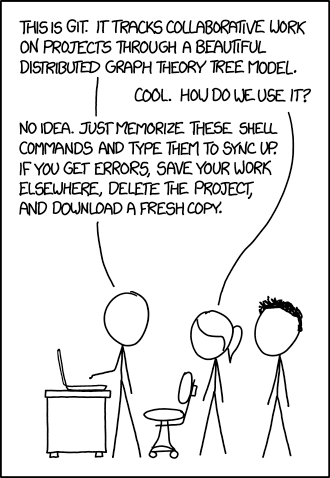
\includegraphics[height=150px]{git_comic}
				\caption{https://xkcd.com/1597/}
				\label{fig1}
			\end{figure}
		\end{frame}

			\begin{frame}
				\frametitle{Weitere Informationen}
					\begin{block}{Ausblick}
						\begin{itemize}
							%\item Branches
							\item Rebasing (Versionsgeschichte umschreiben)
							\item uvm.
						\end{itemize}
					\end{block}
					\begin{block}{Weitere Materialien}
						\begin{itemize}
							\item Offizielle Dokumentation: \href{https://git-scm.com/doc}{https://git-scm.com/doc}
							\item Interaktives Tutorial von GitHub: \href{https://try.github.io/}{https://try.github.io/}
							\item \textit{Pro Git} Buch: \href{https://git-scm.com/book/de}{https://git-scm.com/book/de}
						\end{itemize}
					\end{block}
			\end{frame}
	
\end{document}
